\documentclass{report}

\usepackage{ressources/packages/miseEnPage}
\usepackage{ressources/vocabulaire/vocabulaire}

\pdfminorversion=4
\usepackage[francais]{babel}
\usepackage[utf8]{inputenc}
\usepackage[T1]{fontenc}
\usepackage{graphicx}
\usepackage{fancyhdr}
\usepackage{pdfpages}
\usepackage{float}
\usepackage{diagbox}
\usepackage[urlcolor=blue, linkcolor=black,linktoc=all, colorlinks=true]{hyperref}
\usepackage[left=2.5cm, right=2.5cm, top=2.5cm, bottom=2.5cm, headheight=15pt]{geometry}
\usepackage[final]{pdfpages}
\usepackage{helvet}
\usepackage{lscape}
\usepackage{wasysym}
\usepackage[multidot]{grffile}

\renewcommand{\familydefault}{\sfdefault}

\makeatletter
\def\@makechapterhead#1{% chapter
  \vspace*{5\p@}
  {
    \parindent \z@ \raggedright \normalfont
    \ifnum \c@secnumdepth >\m@ne
    \huge\bfseries \@chapapp\space \thechapter
    \par\nobreak
    \vskip 5\p@
    \fi
    \interlinepenalty\@M
    \Huge \bfseries #1\par\nobreak
    \vskip 10\p@
    \thispagestyle{fancy}% Permet d'ajouter l'entête de pied de page
  }
}

\def\@schapter#1{
  \if@twocolumn
  \@topnewpage[\@makeschapterhead{#1}]
  \else
  \@makeschapterhead{#1}
  \@afterheading
  \fi
}

\def\@makeschapterhead#1{% chapter*
  \vspace*{5\p@}
  {
    \parindent \z@ \raggedright
    \normalfont
    \interlinepenalty\@M
    \Huge \bfseries  #1\par\nobreak
    \vskip 10\p@
    \thispagestyle{fancy} % Permet d'ajouter l'entête de pied de page
  }
}
\makeatother


\usepackage[utf8]{inputenc}
\usepackage[T1]{fontenc}
\usepackage[francais]{babel}
\usepackage{graphicx, titlesec}

\begin{document}
\lstset{ %
  backgroundcolor=\color{white},   % choose the background color; you must add \usepackage{color} or \usepackage{xcolor}
  basicstyle=\footnotesize,        % the size of the fonts that are used for the code
  breakatwhitespace=false,         % sets if automatic breaks should only happen at whitespace
  breaklines=true,                 % sets automatic line breaking
  captionpos=b,                    % sets the caption-position to bottom
  commentstyle=\color{mygreen},    % comment style
  deletekeywords={...},            % if you want to delete keywords from the given language
  escapeinside={\%*}{*)},          % if you want to add LaTeX within your code
  extendedchars=true,              % lets you use non-ASCII characters; for 8-bits encodings only, does not work with UTF-8
  frame=single,                    % adds a frame around the code
  keepspaces=true,                 % keeps spaces in text, useful for keeping indentation of code (possibly needs columns=flexible)
  keywordstyle=\color{blue},       % keyword style
  language=C++,                    % the language of the code
  morekeywords={*,...},            % if you want to add more keywords to the set
  numbers=left,                    % where to put the line-numbers; possible values are (none, left, right)
  numbersep=5pt,                   % how far the line-numbers are from the code
  numberstyle=\tiny\color{mygray}, % the style that is used for the line-numbers
  rulecolor=\color{black},         % if not set, the frame-color may be changed on line-breaks within not-black text (e.g. comments (green here))
  showspaces=false,                % show spaces everywhere adding particular underscores; it overrides 'showstringspaces'
  showstringspaces=false,          % underline spaces within strings only
  showtabs=false,                  % show tabs within strings adding particular underscores
  stepnumber=2,                    % the step between two line-numbers. If it's 1, each line will be numbered
  stringstyle=\color{mymauve},     % string literal style
  tabsize=2,                       % sets default tabsize to 2 spaces
  title=\lstname                   % show the filename of files included with \lstinputlisting; also try caption instead of title
} 

\couverture{}
\pagestyle{pageNormale}

\setcounter{page}{1}
\tableofcontents{}
\chapter{Diagramme de cas d'utilisation}
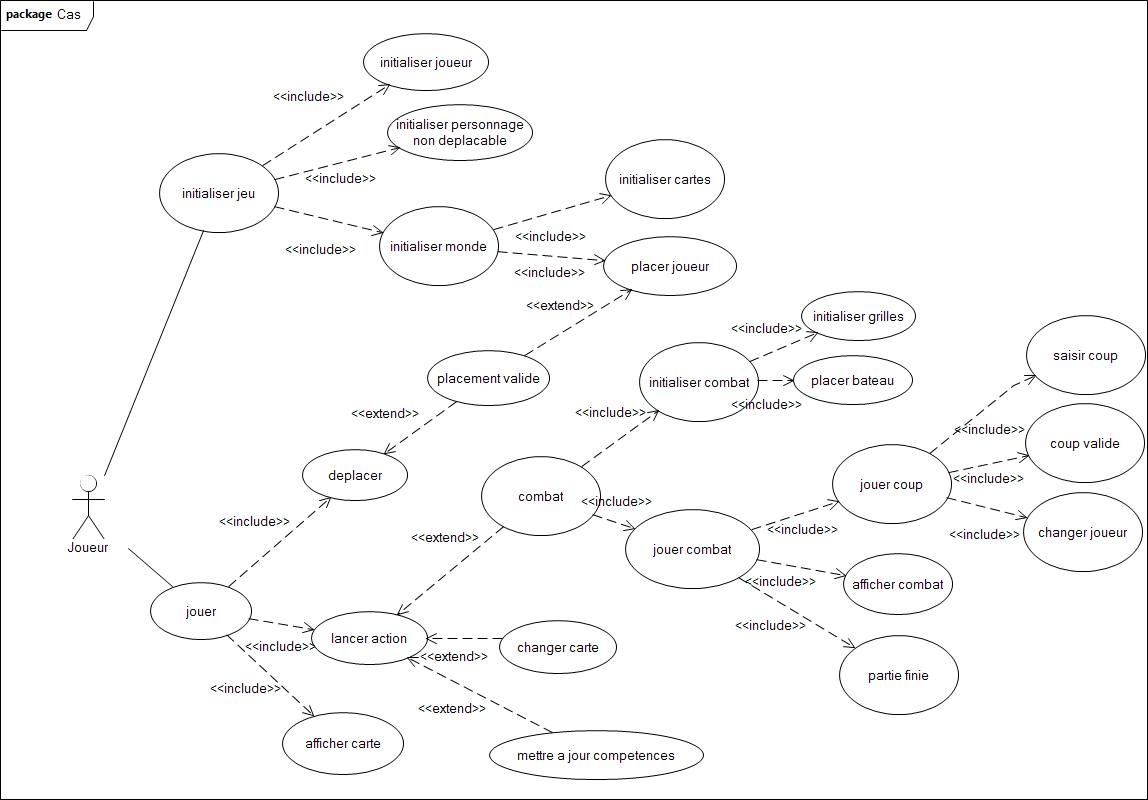
\includegraphics[width=\textwidth,height=\textheight,keepaspectratio]{../graph/DiagrammeDeCasDUtilisation.png}

\chapter{Diagramme de classes}
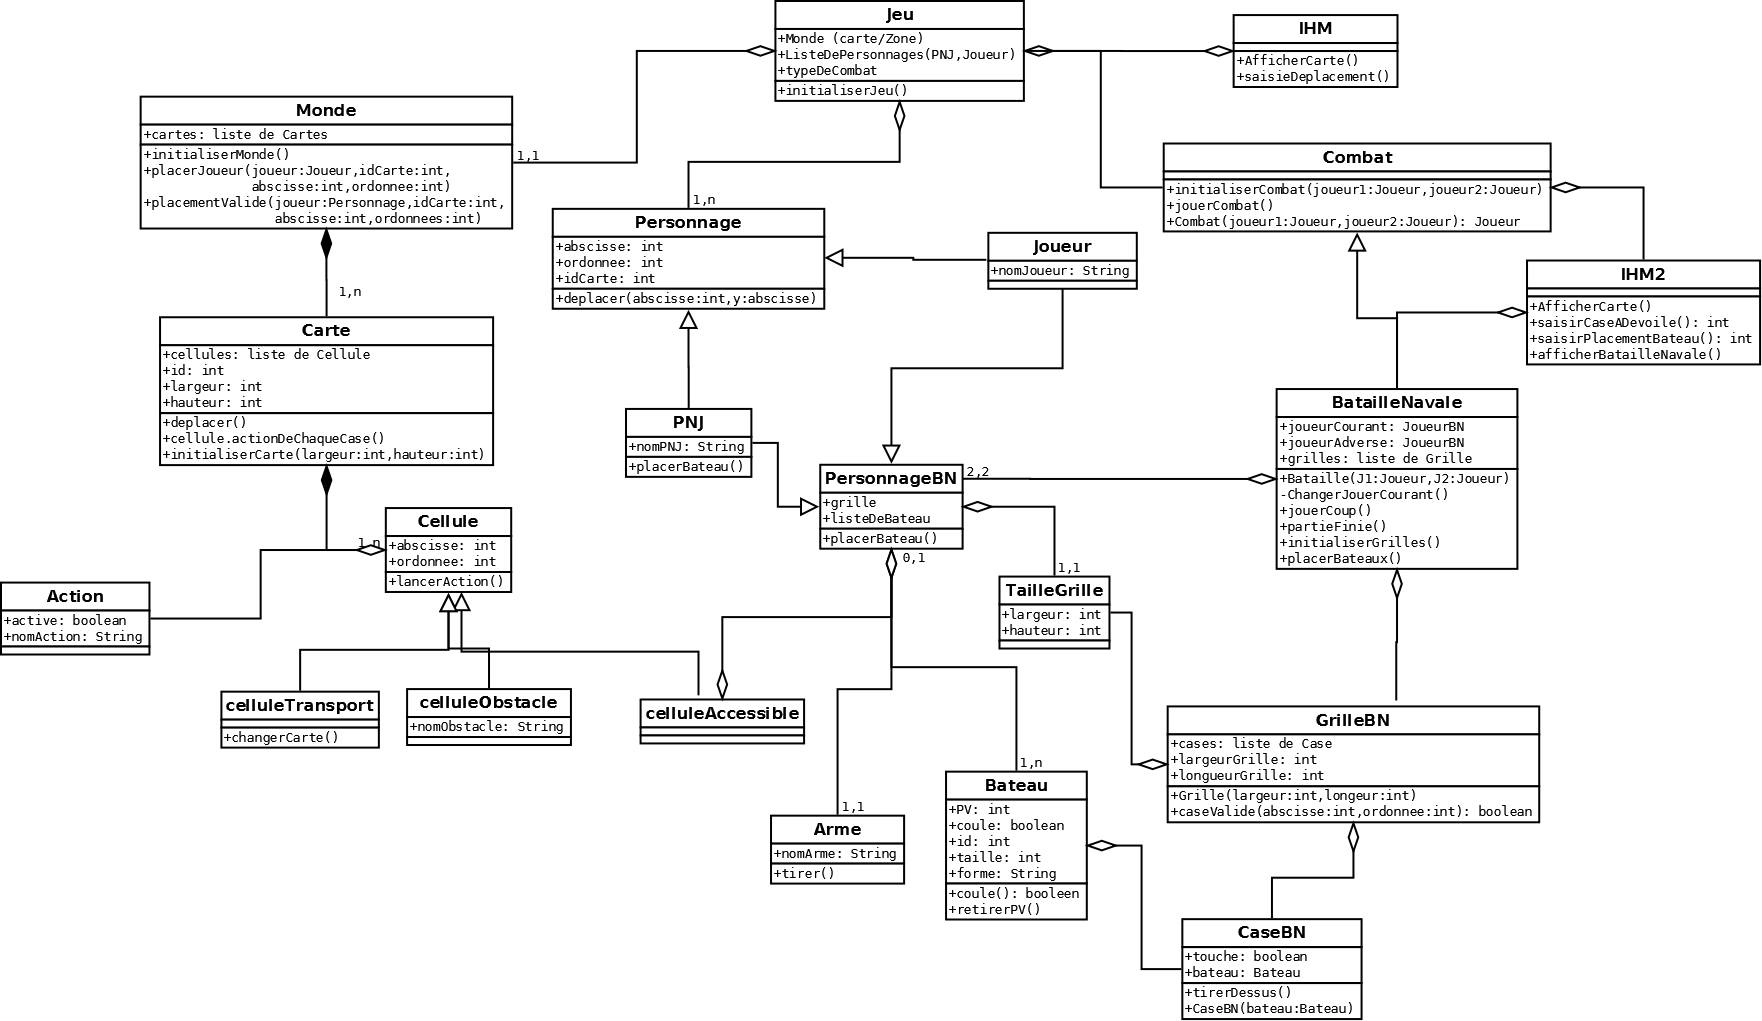
\includegraphics[width=\textwidth,height=\textheight,keepaspectratio]{../graph/DiagrammeDeClasses.jpg}

\chapter{Scénarios}
    \section{InitialiserJeu}
        Pour initialiser le jeu, il nous faudra initialiser:
        \begin{itemize}
            \item Les personnages non-déplacables
            \item Le joueur qui peut être soit un humain soit une IA
            \item Le monde
        \end{itemize}
        \subsection{InitialiserJoueursNonDeplacables}
            Pour chaque Personnage Non Deplacable, on va initialiser leur différents attributs:
            \begin{itemize}
                \item Leur \textbf{nom} a une valeur donnée.
                \item Leur \textbf{position} a NULL.
                \item Leur \textbf{carte} a NULL.
            \end{itemize}
            Leur position et leur carte seront redéfinis par la suite, lorsque le monde aura été crée.\\
        \subsection{InitialiserJoueur}
            Le joueur pourra être de 2 types diff\'erents:
            \begin{itemize}
                \item Un joueur humain.
                \item Une IA.
            \end{itemize}
            Puis nous initialiserons notre heros de la même manière que les Personnage Non Deplacables, avec une specification de sa m\'ethode de jouer en fonction de son type (IA ou humain).
        \subsection{InitialiserMonde}
            Pour chaque carte du monde, nous initialiserons cette carte, puis nous placerons les joueurs.
            \subsubsection{InitialiserCarte}
                Pour initialiser la carte, on récupèrera la taille (largeur et hauteur).\\
                Ensuite, on initialisera chaque cellule de cette carte d'une des trois manières possibles:
                \begin{itemize}
                    \item Cellule \textbf{transport}.
                    \item Cellule \textbf{obstacle}.
                    \item Cellule \textbf{accessible}.
                \end{itemize}
            \subsubsection{PlacerJoueurs}
                Pour chaque joueur déjà initialisé, on le placera a sa position dans sa carte, en vérifiant que le placement est valide.\\
                De plus, on mettra a jour ses attributs position et carte.
                \subsubsection{PlacementValide}
                    Pour le placement du joueur, on vérifiera:
                    \begin{itemize}
                        \item Si la nouvelle position est dans la carte.
                        \item Si la nouvelle cellule est accessible, et ne contient pas déjà un personnage.
                    \end{itemize}
    \section{Jouer}
        On \textbf{affiche la carte}, puis on propose au \textbf{joueur de se déplacer}.\\
        On \textbf{lancera une action} si besoin est.
        \subsection{AfficherCarte}
            Pour afficher la carte, on commence par récuperer la carte du Héros.\\
            Une fois récupérée, chaque cellule sera affichée.
        \subsection{Déplacer}
            Pour déplacer le héros, on demandera tout d'abord au joueur de \textbf{choisir son déplacement}, puis on vérifiera que \textbf{ce déplacement est valide}.\\
            Une fois cette vérification faite, on appliquera le déplacement.
            \subsubsection{SaisieDéplacement}
                Le joueur humain rentrera les coordonnées du déplacement souhaité.
	    Le joueur IA choisira les coordonnées de son déplacement. 
            \subsubsection{PlacementValide}
                Ce scénario reste le même que celui précedemment detaillé.
        \subsection{LancerAction}
            Si la cellule dans laquelle se trouve maintenant le héros est associée à une action, alors cette action est effectuée.
    \section{Combat}
        Pour jouer un combat, on commence par \textbf{initialiser le combat}, pour ensuite \textbf{jouer des coups} tant que le jeu n'est pas terminé.
        \subsection{InitialiserCombat}
            Pour initialiser le combat, qui est dans notre cas une Bataille Navale, il faut:
            \begin{itemize}
                \item Initialiser le plateau.
                \item Placer les bateaux.
            \end{itemize}
            \subsubsection{InitialiserGrilles}
                Pour chacun des deux joueurs en lice, on va initialiser sa grille. On r\'ecupèrera donc la taille de sa grille, pour ensuite créer toutes les cases.
            \subsubsection{PlacerBateaux}
                Une fois les grilles initialisées, chacun des joueurs placera ses bateaux.\\
                Dans le cas des Personnage Non Deplacable, cela fait automatiquement, alors que dans le cas du héros une saisie sera demandée.
                \subsubsection{ChangerCarte}
                    Si le héros se trouve sur une cellule transport, il est d\'eplacé sur la carte correspondante, aux coordonnées corespondantes.
                \subsubsection{MettreAJourComp\'etences}
                    À l'issue d'un combat, le joueur victorieux r\'ecupère des comp\'etences suppl\'ementaires.
                \subsubsection{JouerCombat}
                    Détails ci-dessous.
        \subsection{JouerCombat}
            À chaque tour de jeu, on \textbf{affiche les deux grilles}, puis le joueur courant \textbf{joue son coup} tant que la \textbf{partie n'est pas finie}.
            \subsubsection{AfficherCombat}
                On affiche deux grilles:
                \begin{itemize}
                    \item La grille du joueur courant (compl\'etement dévoilée)
                    \item La grille du joueur adverse (dont seule les cases déjà visées seront montrées)
                \end{itemize}
            \subsubsection{JouerCoup}
                Jouer un coup consiste en:
                \begin{itemize}
                    \item Une choix de coup
                    \item Une vérification de la validité du coup
                    \item Le placement du coup
                    \item Le changement du joueur courant
                \end{itemize}
                    \subsubsection{SaisirCoup}
                        Le joueur courant humain saisie les coordonnées du tir tandis que l'IA calcule les coordonnées de son coup. 
                    \subsection{CoupValide}
                        On vérifie que:
                        \begin{itemize}
                            \item les coordonnées appartiennent bien à la grille.
                            \item La case n'a pas déjà été visée.
                        \end{itemize}
                    \subsection{PlacerCoup}
                        On effectue les changements associés à ce coup sur la grille:
                        \begin{itemize}
                            \item Rév\'elation de la case visée.
                            \item Si cette case contient un bateau auquel retire un point de vie.
                        \end{itemize}
                    \subsection{ChangerJoueur}
                        Le joueur courant devient le joueur adverse et vice-versa.
            \subsubsection{PartieFinie}
                On vérifie si tous les bateaux d'un des joueurs ont été coulés.

\chapter{Diagrammes de sequences}
    \section{InitialisationMonde}
        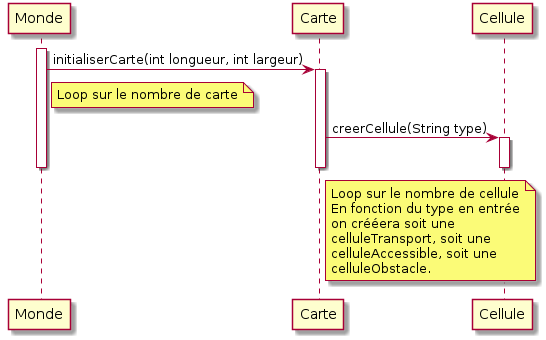
\includegraphics[scale=0.5]{../graph/DiagrammeSequenceInitialisationMonde.png}
    \section{Initialisation}
        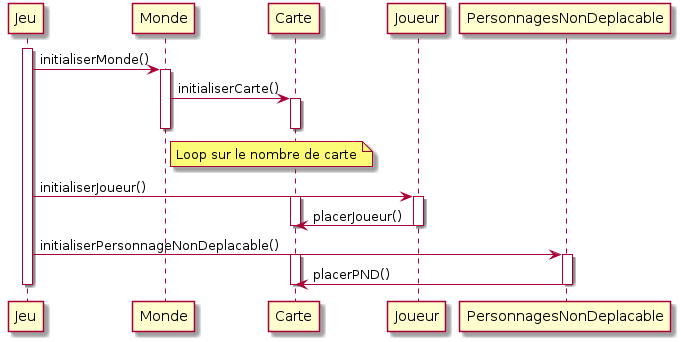
\includegraphics[scale=0.5]{../graph/DiagrammeSequenceInitialisation.png}
    \section{AfficherCarte}
        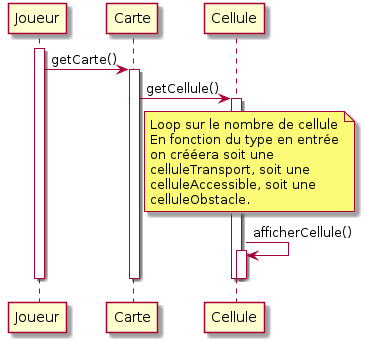
\includegraphics[scale=0.5]{../graph/DiagrammeSequenceAfficherCarte.png}

\chapter{Tests Unitaires}
    Pour chacun de nos tests, nous avons créés un Main qui instanciait l'objet à l'aide de ses différents constructeurs et qui testait l'ensemble des fonctions de la classe à l'aide de ses différents cas au limite.
    \section{TestActionChangementCarte.cpp}
        \subsection{Description}
            On va tester si un personnage est bien transporté comme indiqué dans le constructeur de notre ActionChangementCarte. On verifiera par la même occasion le texte d'interaction de l'action, et voir si l'on peut changer son attribut "Active".
        \subsection{Code}
    \section{TestActionCombat.cpp}
        \subsection{Description}
            On va tester si le personnage donné dans le constructeur est bien celui présent dans l'action.
        \subsection{Code}
    \section{TestActionVide.cpp}
        \subsection{Description}
            On verifie que le texte donné en constructeur est bien celui stocké et affiché dans l'appel de la méthode.
        \subsection{Code}
    \section{TestArmeChercheuse.cpp}
        \subsection{Description}
            On va verifier l'état de la grille après des coup d'arme chercheuse.\\
            On verifie entre autre que les coups ne touchent que des bateaux, et ce même si la coordonnées donnée ne correspond pas.
        \subsection{Code}
    \section{TestArmeClassique.cpp}
        \subsection{Description}
            On verifie l'état de la grille après chaque coup d'arme classique.\\
            On verifie de plus que le bateau est bien touché, pui coulé, avec l'utilisation de cette arme
        \subsection{Code}
    \section{TestArmeCroix.cpp}
        \subsection{Description}
            On verifie l'état de la grille après chaque coup d'arme croix.\\
            On verifie entre autre si les coups sur le bords ne touchent que les cases à l'interieur de la grille, et que les bateau touché par les "bras" de la croix le sont bien.
        \subsection{Code}
    \section{TestArmeFatale.cpp}
        \subsection{Description}
            On verifie l'état de la grille après chaque coup d'arme fatale.\\
            On regarde si lors des coups dans l'eau, une seule case est touchée, alors que si on touche un bateau, ce dernier est bien directement coulé.
        \subsection{Code}
    \section{TestBadgeFinal.cpp}
        \subsection{Description}
            On verifie juste si le badge final met bien fin au jeu.
        \subsection{Code}
    \section{TestBatailleNavale.cpp}
        \subsection{Description}
            On simule une parte complète de bataille navale entre deux IA (Une IA et IA Avancée) avec des taille de grille différentes, des flottes différentes et des armes différentes.\\
            Le bon déroulement de la partie assure le fonctionnement de cette classe
        \subsection{Code}
    \section{TestBateau.cpp}
        \subsection{Description}
            On verifie l'état du bateau après plusieur de retrait de PV. On veut verifier que le bateau passe a coulé une fois seulement que les PVs sont décendus à zéro.
        \subsection{Code}
    \section{TestCase.cpp}
        \subsection{Description}
            On verifie qu'en plaçant un bateau sur une case, le premier tir sur la case retire bien des PV, mais les suivants non.
        \subsection{Code}
    \section{TestCelluleAccessible.cpp}
        \subsection{Description}
            On verifie si le placement d'un personnage sur une cellule accessible est possible.\\
            Dans ce cas, on verifie donc que le bon personnage est ajouté, et on verifie que cette cellule ne contient pas d'action
        \subsection{Code}
    \section{TestCelluleChangementCarte.cpp}
        \subsection{Description}
            On instancie une CelluleChangementCarte, et on verifie que ses paramètre sont bien ceux souhaités
        \subsection{Code}
    \section{TestCelluleCombat.cpp}
        \subsection{Description}
            On crée une cellule combat et on verifie que le personnage du constructeur est bien celui présent sur la case.\\
            On verifie si la cellule est bien inaccessible une fois le personnage dessus
        \subsection{Code}
    \section{TestCelluleObstacle.cpp}
        \subsection{Description}
            On verifie que la cellule est bien innaccessible et que son type est le bon
        \subsection{Code}
    \section{TestControleurBN.cpp}
        \subsection{Description}
            On instancie un controleur BN prenant en paramèter une bataille navale, a laquelle on ajoute deux personnage.\\
            Après le bon deroulement de la première partie, on re-initialise une seconde fois la bataille navale avec de nouveaux joueurs et on verifie le second bon déroulement de la partie.
        \subsection{Code}
    \section{TestCoordonnees.cpp}
        \subsection{Description}
            On instancie tour a tour des coordonnées nulle, puis vide, puis par recopie et on teste toutes les méthodes sur ces dernières
        \subsection{Code}
    \section{TestGrille.cpp}
        \subsection{Description}
            On instancie différentes grilles pour effectuer les tests de placements.
        \subsection{Code}
    \section{TestIHMBN.cpp}
        \subsection{Description}
            On crée une bataille navale et on simule une partie de bataille navale grâce a des fonctions copiée-collée de controleurBN.
        \subsection{Code}
    \section{TestInventaire.cpp}
        \subsection{Description}
            On Instancie deux inventaires, auxquels on ajoute des badges finaux, et on teste leurs tailles en fin de test.
        \subsection{Code}
    \section{Test.cpp}
        \subsection{Description}
        \subsection{Code}
    \section{Test.cpp}
        \subsection{Description}
        \subsection{Code}
    \section{Test.cpp}
        \subsection{Description}
        \subsection{Code}
    \section{Test.cpp}
        \subsection{Description}
        \subsection{Code}
    \section{Test.cpp}
        \subsection{Description}
        \subsection{Code}
    \section{Test.cpp}
        \subsection{Description}
        \subsection{Code}
    \section{Test.cpp}
        \subsection{Description}
        \subsection{Code}
    \section{Test.cpp}
        \subsection{Description}
        \subsection{Code}
    \section{Test.cpp}
        \subsection{Description}
        \subsection{Code}
    \section{Test.cpp}
        \subsection{Description}
        \subsection{Code}
    \section{Test.cpp}
        \subsection{Description}
        \subsection{Code}
    \section{Test.cpp}
        \subsection{Description}
        \subsection{Code}
    \section{Test.cpp}
        \subsection{Description}
        \subsection{Code}
    \section{Test.cpp}
        \subsection{Description}
        \subsection{Code}
    \section{Test.cpp}
        \subsection{Description}
        \subsection{Code}
    \section{Test.cpp}
        \subsection{Description}
        \subsection{Code}
    \section{Test.cpp}
        \subsection{Description}
        \subsection{Code}
    \section{TestTailleGrille.cpp}
        \subsection{Description}
            On instancie 3 grilles (1 nulle, une non nulle, une par recopie) et on teste les différentes méthode sur les 3.
        \subsection{Code}

\chapter{Méthodes de travail}
    Ayant décidés de faire notre projet à sept, il nous à fallu élaborer des méthodes de travail permettant une bonne communication et une bonne coordination. Tout d'abord, nous avons organisé plusieurs réunions d'équipe afin de poser les bases du projet pour que tous les membres soient d'accord sur la conception, le sens des différentes entités, le déroulement du jeu ... Puis nous nous sommes accordés sur l'utilisation de certains logiciels que nous allons vous présenter ici:\\
    \section{GIT}
        Pour la répartition des fichiers, nous avons utilisé le logiciel \textbf{GIT}.\\
        Ce dernier à permis un partage optimal de fichier, facilitant l'envoi et réception de ces derniers.\\
        En plus de cela, GIT nous a permis de travailler en simultané à partir de plusieur poste, sur les même ficheirs et ce, sans aucun problème.\\
    \section{PlantUML}
        Nous avons utilisé \textbf{PlantUML} afin de concevoir le diagramme de classes, de séquence, ainsi que celui de cas d'utilisation.\\
        Ce dernier permet de saisir les diagrammes sous forme de texte très simplement (Via l'utilisation de flèches majoritairement). \\
        Grâce à cela, nous pouvions même modifier en simultané les diagramme de classe grâce à git, à condition de regenerer ces images avant chaque PDF (Le tout fait grâce à un \textbf{Makefile}).\\
    \section{Script génération diagramme de classe}
        Pour optimiser noter temps de travail, et du fait que notre structure de données était imposante, nous avons décidé de prendre un temps pour créer un script nous permettant de generer automatiquement le diagramme de classe en fonction de notre avancée du code dans le CPP et le HPP.\\
        Cela fonctionne grâce à un \textbf{script BASH}, qui trace les classes et leurs liaisons (indiquées dans un fichier externe), mais surtout de maintenir à jour les méthodes et attributs de nos classes. \\
        En plus de cela, nous avons optimisé le code et avons ajouté la possibilité d'indiquer l'avancement du code d'une méthode via des balises //TODO (À faire), //WIP (Work In Progress <=> En cours) et //DONE (Terminé), et que cela soit retranscrit sur le graphique.
    \section{Doxygen}
        Pour la documentation du projet, nous avons utilisé le logiciel \textbf{Doxygen}. Ce dernier nous a permis de pouvoir generer simplement une documentation HTML et PDF. \\
        En contrepartie, nous devions simplement commenter dans chaque HPP chacun des membres présent, en y specifiant ses composant et une description.

\chapter{Répartition des tâches}

\chapter{Conclusions personnelles}
    \section{Thibaut Chavane}
        Ce travail a été intéressant, tant par le travail qu'il représentait en lui-même (coder un jeu avec de nombreuses possibilités, et deux grandes sous-parties quasiment indépendantes), mais aussi par les méthodes auxquelles nous avons eu recours au cours du semestre, comme par exemple l'utilisation de Git, Doxygen, PlantUML. \\
        De plus, le nombre conséquent de membres du groupe nous a permis de nous entraîner à la gestion d'une équipe, plus que lorsqu'on effectue des projets en groupes plus réduits (de deux ou trois étudiants par exemple).
    \section{Clémentine Cavaroc}
        Ce projet nous a à tous paru ambitieux car il représentait une masse de travail considérable, mais grâce à une répartition des tâches efficace et une bonne gestion du temps, nous sommes parvenus à mener à bien ce projet dans les temps. \\
        L'avantage d'avoir réparti les tâches en fonction des niveaux en programmation de chacun est que chacun a pu progresser et contribuer à l'avancement global du projet en même temps, ce qui est après tout le but de chaque projet.
    \section{Léo Lhuissier}
        L'idée de créer un jeu imbriqué dans une autre a été très instructif car c'est quelque chose que nous n'avions pas eu l'occasion d'expérimenter auparavant. \\
        De plus, le fait d'avoir été un groupe plutôt nombreux nous a permis de nous entraîner à la gestion d'une équipe, ce qui fait partie intégrante du métier d'ingénieur.
    \section{Bastien Laine}
        Lors de ce projet, j'ai eu l'occasion de découvrir de nouvelle technologies, ainsi que de continuer mon apprentisage sur d'autre. \\
        De plus, une chose non quantitative que m'aura appris ce projet est le travail en équipe en plus grand nombre. En effet jusqu'ici, aucune matière ne nous à poussé à travailler à 7, et ce sur une tâche d'une empleur aussi conséquente. Cela nous a permis de mettre en place de nouvelle méthode de travail, de division de travail, ou encore de communication, qui jusque là n'avaient pas été necessaire. \\
        Il est clair que le projet aurait pu être amélioré, nottament sur une plus grande "généralité" du code ( Par exemple via des classe IHMCombat, ControleurCombat, ect...). \\
        Cependant à notre niveau, le travail est satisfaisant, surtout de par le fait que nous avons pu implémenter de nouvelle Arme, ou IA de manière très rapide, montrant l'efficacité de la généralite de notre code.

\pageQuatriemeCouverture{}
\end{document}
